\input{../header}
\usepackage{tikz}
\usetikzlibrary{shapes, arrows}
\usepackage[T1]{fontenc}
\usepackage{algorithm}
\usepackage{algpseudocode}
\usepackage{array}
\newcolumntype{C}[1]{>{\centering\let\newline\\\arraybackslash\hspace{0pt}}m{#1}}
\tikzset{vertex/.style={
        circle,
        draw=DarkBlueContour,
        fill=LightBlueFill,
        minimum size=20pt,
        inner sep=0pt,
    },
    % The style for edges
    edge/.style={thick, black!70}}

\begin{document}

\definecolor{DarkBlueContour}{RGB}{0, 0, 150}
\definecolor{LightBlueFill}{RGB}{173, 216, 230}

% Change the following values to true to show the solutions or/and the hints
\ShowSolutiontrue
\ShowConseiltrue
\titre
\cours{Algorithmes de graphes}

Le but de cette séance est de comprendre le fonctionnement des graphes et d'appliquer des algorithmes courants sur des graphes simples. \\

Le code présenté dans les énoncés se trouve sur Moodle, dans le dossier \lstinline{code}. Le temps indiqué (\faClock) est à titre indicatif.

\section{Parcours en largeur — Breadth-First Search}

\begin{Exercice}[10 minutes]  \textbf{Adjacency list et adjacency matrix : Python}\\
    L'adjacency list (ou liste de contiguïté) et l'adjacency matrix (ou matrice de contiguïté) sont les deux méthodes dont nous disposons pour représenter un graphe. \newline 
    
    Utilisez ces deux méthodes de représentations pour stocker le graphe ci-dessous dans un programme Python\!: \\
    %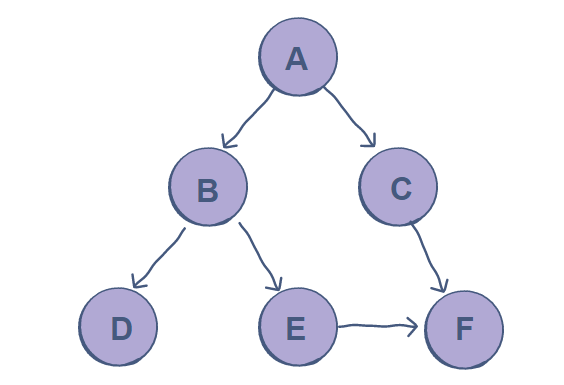
\includegraphics[]{resources/Graphe1.PNG}   
    \begin{center}
        \resizebox{.5\textwidth}{!}{% <------ Don't forget this %
    \begin{tikzpicture}
% --- Draw Vertices (Nodes) ---
    \node[vertex] (D) at (0, 0)  {D};
    \node[vertex] (B) at (1, 1)  {B};
    \node[vertex] (A) at (2, 2)  {A};
    \node[vertex] (E) at (2, 0)  {E};
    \node[vertex] (F) at (4, 0)  {F};
    \node[vertex] (C) at (3, 1) {C};

% --- Draw Edges (Assumed to be a Cycle C_n) ---
    \draw[edge, ->]  (B) -- (D);
    \draw[edge, ->]  (A) -- (B);
    \draw[edge, ->]  (A) -- (C);
    \draw[edge, ->]  (C) -- (F);
    \draw[edge, ->]  (E) -- (F);
    \draw[edge, ->]  (B) -- (E);
    \end{tikzpicture}
        }
\end{center}
    \begin{conseil}
    Pour l'adjacency list, utilisez un dictionnaire Python. Pour l'adjacency matrix, utilisez une liste multidimensionnelle (ou liste contenant une ou plusieurs listes).
    \end{conseil}
    \begin{solution}
        \lstinputlisting[language=python, firstline=1, firstnumber=1, lastline=11]{solutions/graphRepresentation.py}
    \end{solution}

    \begin{solution}
    \lstinputlisting[language=python, firstline=12, firstnumber=12]{solutions/graphRepresentation.py}
    Pour l'adjacency matrix, les indices sont les suivants A=0, B=1, C=2, D=3, E=4, F=5. L'axe 0 de la matrice (verticale), désigne de quel sommet on part, l'axe 1 de la matrice (horizontale), designe vers quel sommet l'arête va.\\
    Si on regarde la première ligne de la matrice, \lstinline{[0,1,1,0,0,0]}, cela correspond à tous les arêtes qui partent de A et vont vers d'autres sommets. Ici B et C, car il y a des 1 aux positions 1 et 2.
    Plus généralement, l'entrée \lstinline{M[i][j]} vaut 1 s'il existe une arête allant du sommet i vers le sommet j, et 0 sinon.\\
    Le fait que le graphe soit dirigé joue un rôle important pour la construction de ces représentations. Par exemple, pour l'adjacency list, B apparaît dans la liste correspondant à la clé A mais l'inverse n'est pas vrai. Cela signifie que l'on peut aller du sommet A au sommet B mais pas du sommet B au sommet A.\\

    \end{solution}

\end{Exercice}


\begin{Exercice}[20 minutes]  \textbf{Breadth-First Search algorithm : Python}\\
    Nous allons maintenant nous intéresser au premier algorithme portant sur les graphes\!: \textbf{Breadth-First Search}. Le but du Breadth-First Search est de trouver tous les sommets atteignables à partir d'un sommet de départ.\\

    Implémentez l'algorithme en suivant les étapes suivantes :\\
\begin{enumerate}
    
    % \item Partez du sommet initial, visitez les sommets adjacents, sauvegardez-les comme \textbf{visités}, insérez-les dans une \textbf{queue}.
    
    % \item Parcourez la \textbf{queue}. Pour chaque élément de la queue, visitez les sommets adjacents. S'ils ne sont pas dans la liste des sommets visités, ajoutez-le à cette dernière et ajoutez-le à la queue. Une fois que cela est fait, supprimez l'élément parcouru de la queue.
    
    % \item Répétez l'étape 2 jusqu'à ce que la queue soit vide.\\

\item Initialisez\!:
\begin{itemize}
    \item une \texttt{file} (queue FIFO — de type liste) qui contient initialement le sommet de départ.
    \item une liste, appelée \texttt{visited}, de sommets visités qui contient initialement le sommet de départ.
    \item une liste, appelée \texttt{order}, qui stocke l'ordre d'enlèvement de la \texttt{file} — sommets proches au sommet de départ au début de la liste.
\end{itemize}

\item Tant que la \texttt{file} n'est pas vide, répétez les specifications suivantes\!:
\begin{enumerate}
    \item Retirez le premier sommet de la file (utilisez \texttt{pop}) et appelez-le $u$. 
    \item Ajoutez $u$ à \texttt{order}
    \item Pour chaque sommet adjacent $v$ de $u$\!: si $v$ n'est pas dans \texttt{visited}, alors :
        \begin{itemize}
            \item Insérez $v$ à la fin de la \texttt{file}.
            \item Insérez $v$ à la fin de \texttt{visited}.
        \end{itemize}
\end{enumerate}

\item Quand la \texttt{file} devient vide, tous les sommets atteignables depuis le sommet de départ ont été visités en largeur.
\item Retournez \texttt{order}.
\end{enumerate}

    \begin{conseil}
        Quelques conseils pour l'implémentation de votre algorithme :
        \begin{enumerate}
            \item Utilisez un adjacency list comme définie précédemment à la question 1.
            \item Pour le point (2), utilisez une boucle \lstinline{while} avec la condition appropriée.
            \item Pour parcourir les sommets adjacents, utilisez une boucle \lstinline{for}.
            \item L'algorithme devrait retourner une liste contenant l'ensemble des sommets atteignables.
            \item Vous pouvez utiliser l'image du graphe pour déterminer si l'output de votre l'algorithme est correct.
            % \item Pensez à utiliser deux listes qui contiendront la liste des sommets à visiter et ceux qui restent à visiter.
            \item Vous pouvez utiliser la méthode \lstinline{pop()} pour supprimer un élément d'une liste et retourner l'élément supprimé. Cet élément peut être stocké dans une variable.
        \end{enumerate}
        Référez-vous au pseudo-code présenté en cours.
    \end{conseil}
    \begin{solution}
        \lstinputlisting[language=python]{solutions/BFS.py}
        Si vous avez correctement écrit votre algorithme, l'output de celui-ci avec comme input notre graphe et le sommet B devrait être \lstinline|[ 'B', 'D', 'E', 'F']| et \lstinline|['A', 'B', 'C', 'D', 'E', 'F']| pour B.
    \end{solution}
\end{Exercice}


\section{Arbre couvrant minimum (ACM) — Minimum Spanning tree (MST)}
    Nous allons maintenant nous intéresser à \textbf{l'algorithme de Kruskal}. Ce dernier s'applique uniquement aux \textbf{weighted graphs}~(ou graphes pondérés). Ces derniers sont des graphes où les arêtes ont des poids, représentant par exemple une distance. L'algorithme de Kruskal a pour but de trouver un \textbf{arbre couvrant minimum} (ACM). Un graphe connexe est un graphe dans lequel il existe au moins un chemin entre n'importe quelle paire de sommets. Un arbre couvrant minimum S de G est un sous-graphe connexe de G tel que\!:
    \begin{enumerate}
        \item V' = V, c'est-à-dire que tous les sommets de G sont aussi dans S
        \item (V',E') ne contient pas de cycle (pas de cycle dans S)
        \item S est le graphe satisfaisant (1) et (2) et ayant la plus petite somme des poids
        \item Pour chaque paire de sommets dans G, S contient le chemin \textit{minimax} entre ces deux sommets. Le chemin \textit{minimax} est un chemin pour lequel le poids de l'arête la plus lourde est minimisé.
    \end{enumerate}
    
    \textbf{\\}
    
\begin{Exercice}[5 minutes] \textbf{Algorithme de Kruskal\!: Papier}\\
    Appliquez l'algorithme de Kruskal au graphe suivant\!:\\
    \begin{center}
    \resizebox{.5\textwidth}{!}{% <------ Don't forget this %
    \begin{tikzpicture}
% --- Draw Vertices (Nodes) ---
    \node[vertex] (A) at (0, 0)     {A};
    \node[vertex] (B) at (0, 2)     {B};
    \node[vertex] (C) at (1.73, 1)  {C};
    \node[vertex] (D) at (3.46, 0)  {D};
    \node[vertex] (E) at (3.46, 2)  {E};
    \node[vertex] (F) at (5.196, 1)  {F};

% --- Draw Edges (Assumed to be a Cycle C_n) ---
    \draw[edge, -]  (A)-- node[midway, left]  {4} (B);
    \draw[edge, -]  (B)-- node[midway, above] {4} (C);
    \draw[edge, -]  (A)-- node[midway, below] {2}  (C);
    \draw[edge, -]  (C)-- node[midway, above] {3} (E);
    \draw[edge, -]  (C)-- node[midway, below] {2} (D);
    \draw[edge, -]  (C)-- node[midway, above] {4} (F);
    \draw[edge, -]  (E)-- node[midway, above] {3}  (F);
    \draw[edge, -]  (D)-- node[midway, below] {3} (F);
\end{tikzpicture}
}
\end{center}
    \begin{conseil}
        L'algorithme de Kruskal fonctionne de la façon suivante\!:
        \begin{enumerate}
            \item Classer les arêtes par ordre croissant de poids.
            \item Prendre l'arête avec le poids le plus faible et l'ajouter à l'arbre (si 2 arêtes ont le même poids, choisir arbitrairement une des 2).
            \item Vérifiez que l'arête ajoutée ne crée pas de cycle, si c'est le cas, supprimez-la.
            \item Répétez les étapes (2) et (3) jusqu'à ce que tous les sommets aient été atteints.
        \end{enumerate}
        Un arbre couvrant minimum (minimum spanning tree), s'il existe, a toujours un nombre d'arêtes égal au nombre de sommets moins un. Par exemple, ici notre graphe a 6 sommets. L'algorithme devrait donc s'arrêter lorsque 5 arêtes ont été choisies.
    \end{conseil}
    \begin{solution}
        Vous trouverez ci-dessous les étapes de la construction de l'ACM:\\
        \begin{center}
        \begin{tikzpicture}[
    vertex/.style={
        circle,
        draw=DarkBlueContour,
        fill=LightBlueFill,
        minimum size=20pt,
        inner sep=0pt,
    },
    edge/.style={thick, black!70}
]
    % Top-left graph
    \begin{scope}[shift={(0, 2)}]
        % **BORDER FOR Étape 1**
        \draw[dashed, red] (-0.5, -0.5) rectangle (5.7, 3); 
        
        \node[anchor=south] at (2.598, 2.5) {\textbf{Étape 1}};
        \node[vertex] (A1) at (0, 0)     {A};
        \node[vertex] (B1) at (0, 2)     {B};
        \node[vertex] (C1) at (1.73, 1)  {C};
        \node[vertex] (D1) at (3.46, 0)  {D};
        \node[vertex] (E1) at (3.46, 2)  {E};
        \node[vertex] (F1) at (5.196, 1) {F};

        \draw[edge] (C1)-- node[midway, below] {2} (D1);
    \end{scope}

    % Top-right graph
    \begin{scope}[shift={(6.5, 2)}]
        % **BORDER FOR Étape 2**
        \draw[dashed, red] (-0.5, -0.5) rectangle (5.7, 3);
        
        \node[anchor=south] at (2.598, 2.5) {\textbf{Étape 2}};
        \node[vertex] (A2) at (0, 0)     {A};
        \node[vertex] (B2) at (0, 2)     {B};
        \node[vertex] (C2) at (1.73, 1)  {C};
        \node[vertex] (D2) at (3.46, 0)  {D};
        \node[vertex] (E2) at (3.46, 2)  {E};
        \node[vertex] (F2) at (5.196, 1) {F};

        \draw[edge] (A2)-- node[midway, below] {2} (C2);
        \draw[edge] (C2)-- node[midway, below] {2} (D2);
    \end{scope}

    % Bottom-left graph
    \begin{scope}[shift={(0, -2)}]
        % **BORDER FOR Étape 3**
        \draw[dashed, red] (-0.5, -0.5) rectangle (5.7, 3);
        
        \node[anchor=south] at (2.598, 2.5) {\textbf{Étape 3}};
        \node[vertex] (A3) at (0, 0)     {A};
        \node[vertex] (B3) at (0, 2)     {B};
        \node[vertex] (C3) at (1.73, 1)  {C};
        \node[vertex] (D3) at (3.46, 0)  {D};
        \node[vertex] (E3) at (3.46, 2)  {E};
        \node[vertex] (F3) at (5.196, 1) {F};

        \draw[edge] (A3)-- node[midway, below] {2} (C3);
        \draw[edge] (C3)-- node[midway, above] {3} (E3);
        \draw[edge] (C3)-- node[midway, below] {2} (D3);
    \end{scope}

    % Bottom-right graph
    \begin{scope}[shift={(6.5, -2)}]
        % **BORDER FOR Étape 4**
        \draw[dashed, red] (-0.5, -0.5) rectangle (5.7, 3);
        
        \node[anchor=south] at (2.598, 2.5) {\textbf{Étape 4}};
        \node[vertex] (A4) at (0, 0)     {A};
        \node[vertex] (B4) at (0, 2)     {B};
        \node[vertex] (C4) at (1.73, 1)  {C};
        \node[vertex] (D4) at (3.46, 0)  {D};
        \node[vertex] (E4) at (3.46, 2)  {E};
        \node[vertex] (F4) at (5.196, 1) {F};

        \draw[edge] (A4)-- node[midway, below] {2} (C4);
        \draw[edge] (C4)-- node[midway, above] {3} (E4);
        \draw[edge] (C4)-- node[midway, below] {2} (D4);
        \draw[edge] (D4)-- node[midway, below] {3} (F4);
    \end{scope}

    % Bottom-right graph
    \begin{scope}[shift={(0, -6)}]
        % **BORDER FOR Étape 4**
        \draw[dashed, red] (-0.5, -0.5) rectangle (5.7, 3);
        
        \node[anchor=south] at (2.598, 2.5) {\textbf{Étape 5}};
        \node[vertex] (A4) at (0, 0)     {A};
        \node[vertex] (B4) at (0, 2)     {B};
        \node[vertex] (C4) at (1.73, 1)  {C};
        \node[vertex] (D4) at (3.46, 0)  {D};
        \node[vertex] (E4) at (3.46, 2)  {E};
        \node[vertex] (F4) at (5.196, 1) {F};

        \draw[edge] (A4)-- node[midway, below] {2} (C4);
        \draw[edge] (C4)-- node[midway, above] {3} (E4);
        \draw[edge] (C4)-- node[midway, below] {2} (D4);
        \draw[edge] (D4)-- node[midway, below] {3} (F4);
        \draw[edge] (B4)-- node[midway, below] {4} (C4);
    \end{scope}
\end{tikzpicture}
\end{center}
\end{solution}
\begin{solution}
        L'algorithme s'arrête car tous les sommets ont été atteints. On voit bien que seules 5 arêtes ont été nécessaires. On remarque que l'ACM n'est pas unique dans ce cas comme on aurait pu choisir l'arête verticale tout à gauche du poids 4 au lieu de l'autre arête du poids 4.
        Si on a le choix entre plusieures arêtes qui ont le même poids on peut prendre celle qu'on veut. Si l'arête avec le plus petit poids reli un sommet qui est déjà atteint avant alors on ne l'ajoute pas pour ne pas créer de cycle. \\
        Par exemple après l'étape 4 le plus petit poids (3) serait entre les sommets E et F, mais ils sont déjà reliés avec d'autres arêtes donc on ne prends cette arête.
    \end{solution}
\end{Exercice}
\begin{Exercice}[30 minutes] \textbf{Lecture du code — Algorithme de Kruskal\!: Python}\\
    Vous trouverez ci-dessous l'algorithme de Kruskal implémenté en Python (disponible sur Moodle). Lisez le code afin de vous assurez que vous ayez bien compris le fonctionnement\!:\\
    \lstinputlisting[language=python]{solutions/kruskal.py}
    \begin{conseil}
        La sortie de l'algorithme est\!: \\
        0 - 1: 4 \\ 
        0 - 2: 4 \\
        3 - 4: 3 \\
        5 - 2: 2 \\ 
        5 - 4: 3 \\
        Il se lit comme une liste d'arêtes et de poids de l'arête correspondante.
    \end{conseil}
\end{Exercice}


\begin{Exercice}[10 minutes] \textbf{Social Network Analysis : Papier}\\
    Les graphes peuvent être utilisés pour représenter une multitude de choses.  L'une d'entre elles est la représentation de votre réseau d'amis. Imaginez que vous possédiez une liste de vos amis ainsi que des amis de vos amis (qui ne sont pas nécessairement vos amis). Cette liste peut-être représentée sous forme de graphe. Dans ce graphe\!:
    \begin{enumerate}
        \item  À quoi correspondent les arêtes et les sommets? 
        \item Faut-il utiliser un graphe dirigé?
    \end{enumerate}
    Supposez que vous disposiez d'un graphe des relations sociales. Décrivez comment retrouver les éléments suivants :
    \begin{enumerate}
        \item Votre ami qui a le plus d'amis
        \item Découvrir quels amis à vous se connaissent
        \item Listez vos amis qui pourraient vous présenter quelqu'un que vous ne connaissez pas (ami d'ami qui n'est pas votre ami)
    \end{enumerate}
    Vous voudriez désormais ajouter une nouvelle personne sur ce graphe, mais cette dernière n'est ni votre ami, ni l'ami d'un de vos amis. Quel sera son degré dans le graphe?\\
    
    Retrouvez les éléments (1) à (3) dans le graphe ci-dessous :\\
    % 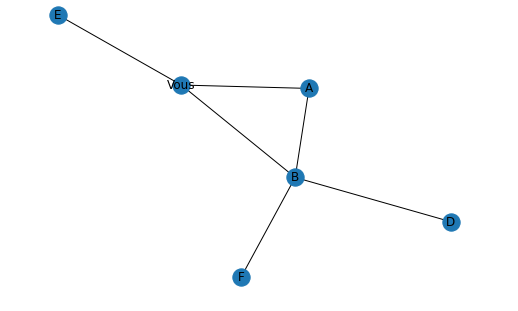
\includegraphics[]{resources/Network1.PNG}
    \begin{center}
    \begin{tikzpicture}[scale=1.4]

        % --- Nodes ---
        \node[vertex] (E)    at (-2,2)      {E};
        \node[vertex] (V)    at (-0.5,1.2)  {\footnotesize Vous};
        \node[vertex] (A)    at (1,1.2)     {A};
        \node[vertex] (B)    at (1,0)       {B};
        \node[vertex] (D)    at (3,0)       {D};
        \node[vertex] (F)    at (1,-1.5)    {F};

        % --- Edges ---
        \draw[edge] (E) -- (V);
        \draw[edge] (V) -- (A);
        \draw[edge] (V) -- (B);
        \draw[edge] (A) -- (B);
        \draw[edge] (B) -- (D);
        \draw[edge] (B) -- (F);

    \end{tikzpicture}
    \end{center}
    \begin{conseil}
        Réfléchissez en terme d'arêtes, de sommets, de degrés et de cycles.
    \end{conseil}

    \begin{solution}
        Dans le graphe des relations sociales, les arêtes correspondent à un lien d'amitié et les nœuds représentent les personnes. Il n'est pas nécessaire d'utiliser un graphe dirigé si l'on considère qu'une relation d'amitié est toujours réciproque.\\
        
        Pour trouver les éléments (1) à (3), il faut raisonner de la façon suivante :
        \begin{enumerate}
            \item Trouvez le sommet relié à vous qui a le degré le plus élevé. Sommet B dans le graphe.
            \item Premièrement, les 2 personnes doivent être mes amis donc reliées à moi, mais de  plus elles doivent être reliées entre elles. Par conséquent, cela correspond à un cycle dans le graphe. Il y a autant d'amis qui se connaissent que de cycles dans le graphe. Ami A et B dans le graphe.
            \item Il ne doit pas y avoir d'arêtes me reliant avec l'ami de mon ami. Sommet B dans le graphe.
        \end{enumerate}
        
        Si l'on ajoute une personne qui n'est ni un ami, ni l'ami d'un ami, alors aucune arête n'est reliée à ce sommet. Par conséquent, ce sommet a un degré 0.
    \end{solution} 
\end{Exercice}

\begin{Exercice}[5 minutes] \textbf{Reconnaître des réseaux semblables}\\
    Supposons maintenant que vous travaillez chez Meta, qui a racheté Whatsapp, et que vous disposiez des deux graphes représentant respectivement Facebook et Whatsapp. Pouvez-vous déterminer visuellement à qui correspondent les individus de Facebook sur Whatsapp?\\
    

\begin{table}[h!]
\centering
\begin{tabular}{|c|c|}
\hline
\textbf{Graphe de Facebook} & \textbf{Graphe de WhatsApp} \\
\hline
\begin{tikzpicture}[scale=1.6]
    % --- Nodes (positions chosen to match your picture) ---
    \node[vertex] (D) at (-0.5,2) {D};
    \node[vertex] (B) at (0,0.8) {B};
    \node[vertex] (F) at (-1,-0.3) {F};
    \node[vertex] (A) at (1,-1.2) {A};
    \node[vertex] (C) at (1.8,0.5) {C};
    \node[vertex] (E) at (3,0.8) {E};

    % --- Edges ---
    \draw[edge] (D) -- (B);
    \draw[edge] (B) -- (F);
    \draw[edge] (B) -- (A);
    \draw[edge] (B) -- (C);
    \draw[edge] (C) -- (E);
    \draw[edge] (A) -- (C);
\end{tikzpicture}
&
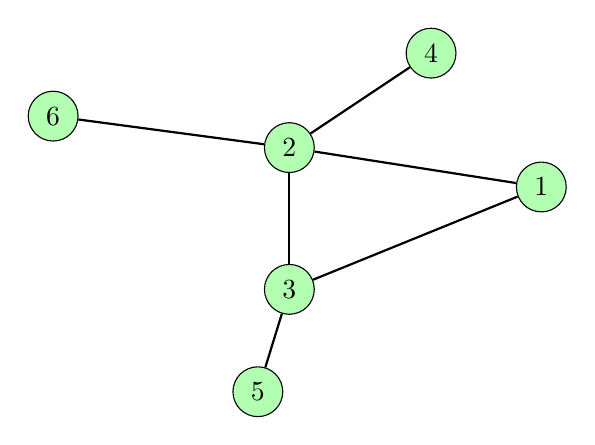
\begin{tikzpicture}[scale=1.0]
    % Green style for the second picture
    \tikzset{
        vertex/.style={
            circle,
            draw=black,
            fill=green!30, % Green theme
            minimum size=18pt,
            inner sep=0pt
        },
        edge/.style={thick}
    }

    % --- Nodes (positioned to match your picture) ---
    \node[vertex] (6) at (-3,1.2) {6};
    \node[vertex] (2) at (0,0.8) {2};
    \node[vertex] (4) at (1.8,2) {4};
    \node[vertex] (1) at (3.2,0.3) {1};
    \node[vertex] (3) at (0,-1) {3};
    \node[vertex] (5) at (-0.4,-2.3) {5};

    % --- Edges ---
    \draw[edge] (6) -- (2);
    \draw[edge] (2) -- (4);
    \draw[edge] (2) -- (1);
    \draw[edge] (2) -- (3);
    \draw[edge] (3) -- (1);
    \draw[edge] (3) -- (5);
\end{tikzpicture}
\\
\hline
\end{tabular}
\end{table}
    
    \begin{conseil}
    Quelques conseils pour vous aider à résoudre cet exercice :
    \begin{enumerate}
        \item Identifiez les sommets des 2 graphes avec des caractéristiques semblables.
        \item Il est possible que les sommets ne soient pas tous identifiables.
    \end{enumerate}
        
    \end{conseil}
    \begin{solution}
        \begin{enumerate}
            \item B correspond à 2 (seul sommet de degré 4)
            \item A correspond à 1 (seul sommet de degré 2 relié au sommet de degré 4)
            \item C correspond à 3 (seul sommet de degré 3)
            \item E correspond à 5 (seul sommet de degré 1 relié au sommet de degré 3)
        \end{enumerate}
        Les sommets D et F et 4 et 6 ne peuvent pas être dissociés. On ne peut donc pas savoir qui correspond à qui.
    \end{solution}
\end{Exercice}


\begin{Exercice}[5 minutes]
Laquelle des affirmations suivantes est correcte?
\begin{conseil}
Un graphe complet est un graphe dans lequel tous les sommets sont adjacents (reliés entre eux). 
\end{conseil}
\begin{enumerate}
\item L'algorithme du parcours en largeur (breadth-first search) ne se termine pas s'il existe un cycle dans le graphe.
\item Pour |G| >> ||G|| (nombre de sommets beaucoup plus grand que nombre d'arêtes), la matrice de contiguïté (adjacency matrix) occupe moins d'espace que la liste de contiguïté (adjacency list).
\item Dans un graphe complet, le nombre d'arêtes est $\frac{n(n-1)}{2}$ et le degré moyen d'un sommet est $n$ où $n=|G|$.
\item Dans l'algorithme de Kruskal, l'instruction \textsc{UNION} est utilisée afin de déterminer si deux sommets sont déjà liés dans l'arbre couvrant minimal et de les relier si ce n'est pas le cas. 
\end{enumerate}
\begin{solution}
    \begin{enumerate}
        \item Fausse: un sommet qui est déjà visité ne sera plus visité.
        \item Fausse: la matrice de contiguïté a une complexité spatiale de $\Theta(V^2)$ tandis que la complexité spatiale de la liste de contiguïté est $\Theta(V+E)$. 
        \item Fausse: dans un graphe complet, chaque sommet est relié aux $n-1$ autres sommets — la première partie de l'affirmation sur le nombre d'arêtes est quand même vraie.
        \item Vraie: cela est exactement l'objectif de \textsc{UNION}. 
    \end{enumerate}
 
\end{solution}
\end{Exercice}

\begin{Exercice}[10 minutes]
Soit le graphe $G$ donné ci-dessous, déterminer le nombre d'ensembles disjoints (disjoint sets) après les deux premiers appels de \textsc{UNION} dans l'algorithme de Kruskal.
\begin{center}
    \begin{tikzpicture}[scale=2]
% --- Draw Vertices (Nodes) ---
    \node[vertex] (A) at (0, 0)  {A};
    \node[vertex] (B) at (1, 1)  {B};
    \node[vertex] (C) at (2, 0)  {C};
    \node[vertex] (D) at (3.5, 0)  {D};

% --- Draw Edges (Assumed to be a Cycle C_n) ---
    \draw[edge]  (B) -- node[midway, below] {1} (C);
    \draw[edge]  (A) -- node[midway, above] {4} (B);
    \draw[edge]  (C) -- node[midway, below] {1} (D);
    \draw[edge]  (B) -- node[midway, above] {2} (D);
    \end{tikzpicture}
\end{center}
    \begin{algorithm}[H]
\caption{MST-KRUSKAL($G, w$)}
\begin{algorithmic}[1]

\State $A \gets \emptyset$

\For{each vertex $v \in G.V$}
    \State \textsc{Make-Set}($v$)
\EndFor

\State sort the edges of $G.E$ into nondecreasing order by weight $w$

\For{each edge $(u, v) \in G.E$, taken in nondecreasing order by weight}
    \If{\textsc{Find-Set}($u$) $\neq$ \textsc{Find-Set}($v$)}
        \State $A \gets A \cup \{(u, v)\}$
        \State \textsc{Union}($u, v$)
    \EndIf
\EndFor

\State \Return $A$

\end{algorithmic}
\end{algorithm}

\begin{solution}
Les deux ensembles sont \{A\} et \{B, C, D\}. Explication: Lors du premier tour de la boucle définie à ligne 6, l'arête BC (ou CD) est examinée. Par conséquent, B et C (ou C et D) sont reliés. Après la deuxième itération, les sommets B, C, et D sont reliés dans l'arbre couvrant minimal — ils appartiennent donc au même ensemble disjoint. A n'est pas encore relié après les deux premières itérations et le sera dans le quatrième tour de la boucle. 
\end{solution}
\end{Exercice}


\end{document}
